\section{Introduzione}
Partiamo dal titolo del corso: Algoritmi paralleli e distribuiti.
Il concetto di algoritmo, quando è nato, non prevedeva la possibilità che gli algoritmi fossero paralleli o distribuiti ma è stato pensato per un unico esecutore.

\begin{definizione}
    Una sequenza finita di istruzioni che sono eseguibili e non ambigue e che portano ad un risultato. Cioè su ogni istanza di input questa sequenza di istruzione termina.
\end{definizione}

Parlando di paralleli e distribuiti, ci riferiamo ad algoritmi che devono essere eseguiti da un \uline{pool di esecutori}. Anche il termine sequenza di istruzioni non è molto corretto in questo contesto ma dobbiamo parlare di \uline{insiemi di istruzioni raggruppate in passi}. Nel caso di algoritmi paralleli avremmo dei passi paralleli dove in ogni passo è possibile avere un set di istruzioni, una istruzione per ogni esecutore. La stessa cosa per i distribuiti. 

Qual'è la differenza tra algoritmi paralleli e algoritmi distribuiti? La differenza sta nel fatto che questi esecutori che lavorano allo stesso momento, possono essere sincronizzati (paralleli) tra di loro o possono essere asincroni (distribuiti)

%Problematiche degli algoritmi sequenziali
\begin{comment}
\paragraph{Poblematiche degli algoritmi sequenziali}
\begin{enumerate}
    \item Progettare: pensare ad un problema e risolverlo. Tecniche note per risolvere algoritmi sequenziali: divide et impera\footnote{Scompone il problema in sotto-problemi e una volta risolti i sotto-problemi li fonde}, programmazione dinamica\footnote{Simile al dividi-et-impera ma entra in gioco anche la memoria dove poter salvare gli esiti parziali dei sotto problemi}, greedy\footnote{Fare la scelta migliore localmente per ottenere il miglior risultato finale}
    \item Valutare le prestazioni: confrontare gli algoritmi tra di loro. Nel caso di algoritmi sequenziali si utilizzano la risorsa tempo e spazio di memoria
    \item Codificare
\end{enumerate}
Analogamente le stesse problematiche possono essere affrontate per algoritmi paralleli e distribuiti
\end{comment}


\paragraph{Algoritmi paralleli}
Far eseguire il compito a più processori, sperando che l’aumento di risorse sia compensato da una diminuzione del tempo di calcolo. I modelli di calcolo in cui siano presenti più processori che lavorano contemporaneamente (sincronizzati con un clock globale) sono detti \textit{paralleli}, così come il modello dotato di un solo processore è detto \textit{sequenziale}
\begin{itemize}
    \item Gli esecutori condividono un clock centrale ed insieme eseguono le istruzioni, vanno all'unisono
    \item Siccome devono lavorare assieme, per portare a termine un algoritmo devono a volte comunicare tra di loro ad esempio dei risultati parziali di qualche operazione che hanno compiuto. Per comunicare tra di loro possono utilizzare la memoria (parallelo a memoria condivisa) oppure hanno a disposizione dei collegamenti/link full-duplex e si spediscono i risultati parziali ottenuti (parallelo a memoria distribuita)
\end{itemize}

Richiamiamo per prima cosa un classico modello di calcolo sequenziale, cioè la macchina RAM; ridotta all’osso, essa consiste di un processore P collegato ad una memoria M attraverso un'unità di accesso. Nei modelli di calcolo parallelo, data la presenza di più processori, un elemento critico è la modalità di comunicazione tra processori. I due casi limite sono rappresentati dal modello a \textit{memoria condivisa} e dal modello a \textit{memoria distribuita}

\begin{figure}[h]
    \centering
    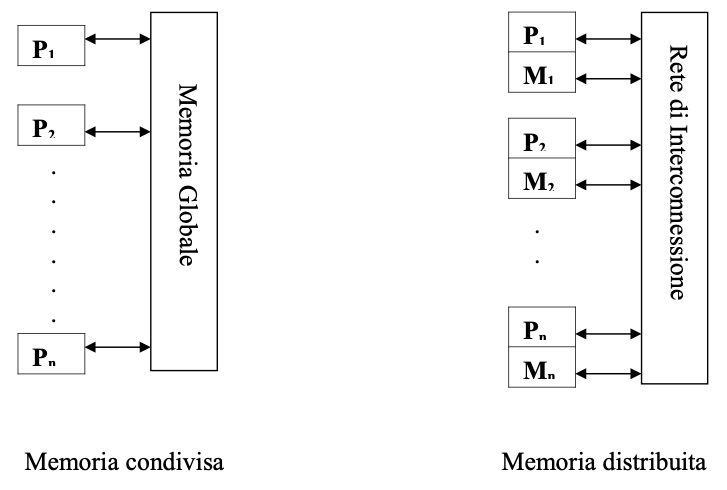
\includegraphics[scale=0.4]{images/memoria_condivisa_distribuita.png}
\end{figure}

Nel modello a memoria condivisa tutti i processori possono accedere alle stesse locazioni di memoria nella stessa unità di tempo. Il meccanismo di comunicazione tra due processori $P_k$ e $P_j$ è molto semplice:
\begin{enumerate}
    \item $P_k$ scrive il messaggio in un’area di memoria
    \item $P_j$ lo legge dalla stessa area
\end{enumerate}
Va segnalato che i processori non sono direttamente connessi e che la comunicazione avviene in tempo costante $O(1)$

Nei modelli a memoria distribuita ogni processore può accedere invece solo alla sua memoria privata (locale). La comunicazione avviene qui attraverso l’invio di messaggi su una rete di interconnessione, che può essere descritta da un grafo i cui vertici sono i processori e i lati rappresentano collegamenti diretti tra processori. \uline{Poiché in tali reti non tutti i processori sono collegati direttamente, non è possibile ipotizzare tempi di comunicazione costanti, contrariamente a quel che succedeva nel caso a memoria condivisa}

Nel parallelo il fattore rilevante è il TEMPO. Valutatiamo il tempo come il numero di clock necessari a far terminare l'algoritmo

\paragraph{Algoritmi distribuiti}
\begin{itemize}
    \item Ognuno ha un proprio clock centrale, con i propri tempi, che non combacia con quello degli altri
    \item Per comunicare tra di loro sono collegati, ma sicuramente possiamo assumere che non hanno una memoria in comune
\end{itemize}

\begin{osservazione}
La comunicazione gioca un ruolo fondamentale e i tempi di sincronizzazione assumono un ruolo principale rispetto ai tempi di esecuzione delle operazioni. La somma di due numeri richiede un semplice clock ma l'attesa di un dato potrebbe richiedere diversi cicli di clock. E' la comunicazione che assume un ruolo più rilevante rispetto al tempo di esecuzione delle operazioni
\end{osservazione}

\uline{Nel distribuito il fattore rilevante è il COORDINAMENTO}.

\paragraph{Esempi di architetture parallele}
\begin{itemize}
    \item Supercomputer: cluster di processori ad elevate prestazioni di calcolo. Questi vengono utilizzati per emulare fenomeni reali, come fenomeni fisici, economici e militari. Simulano sistemi complessi e hanno bisogno di molti processori per il calcolo
    \item GPU: quello che sanno fare molto bene è risolvere operazioni in spazi vettoriali (matrici)
    \item Multicore processor
\end{itemize}

\paragraph{Esempi di architetture distribuite}
\begin{itemize}
    \item Reti di calcolatori connessi a Internet: la rete permette di coprire alte distanze e troveremo i nostri dispositivi di calcolo molto lontani tra di loro. Per questo ci sarà bisogno di un protocollo di comunicazione condiviso che è il \textit{TCP/IP}
    \item Reti mobili: la topologia delle connessioni cambia durante l'esecuzione di un algoritmo. La connessione non è fissata e varia nel tempo
    \item Reti di sensori: piccoli elementi di calcolo che hanno delle capacità limitate e per la maggior parte del tempo stanno in \textit{stand-by} attivandosi con un messaggio di \textit{wake-up} e poi si rimettono in stand-by. Servono per monitorare delle realtà come la temperatura. Hanno bisogno di meccanismi di \textit{wake-up}, \textit{aknowledge}, \textit{recovery}
\end{itemize}

\newpage